% \documentclass{article}

\documentclass[10pt,aps,onecolumn,superscriptaddress]{revtex4-2}

\usepackage[T1]{fontenc}
\usepackage[utf8]{inputenc}
\usepackage[english]{babel}

\usepackage{amsfonts, amsbsy, amssymb, amsmath, graphicx, float}
\usepackage{hyperref}
\hypersetup{
    colorlinks=true,
    linkcolor=blue,
    filecolor=magenta,      
    urlcolor=cyan,
}
% \usepackage{subfigure}
% \usepackage[numbers,sort&compress]{natbib}
%%%%%%%%%%%%%%%%%%%%%%%%%%%%%%%%%%%%%%%%%%%%%%%%%%%%%

\bibliographystyle{apsrev4-2}


\begin{document}

\title{The Cirque Potential Problem - CHAMPS}


\author{Broncio Aguilar Sanjuan}
\email{broncio.aguilarsanjuan@bristol.ac.uk}
\affiliation{School of Mathematics, University of Bristol, \\ Fry Building, Woodland Road, Bristol, BS8 1UG, United Kingdom.}

\author{V\'ictor J. Garc\'ia-Garrido}
\email{vjose.garcia@uah.es}
\affiliation{Departamento de F\'isica y Matem\'aticas, Universidad de Alcal\'a, \\ Alcal\'a de Henares, 28871, Spain.}

\author{Francisco Gonz\'alez Montoya}
\email{fg16704@bristol.ac.uk}
\affiliation{School of Mathematics, University of Bristol, \\ Fry Building, Woodland Road, Bristol, BS8 1UG, United Kingdom.}

\author{Stephen Wiggins}
\email{s.wiggins@bristol.ac.uk}
\affiliation{School of Mathematics, University of Bristol, \\ Fry Building, Woodland Road, Bristol, BS8 1UG, United Kingdom.}





\date{May 2020}



\begin{abstract}

In this paper we explore  

\end{abstract}

\maketitle

\noindent\textbf{Keywords:} Phase space structure, Chemical reaction dynamics, Roaming, Lagrangian descriptors, 

\section{Introduction}


Single VdW potential \cite{Soley2018}. It models the long-range interaction describing dipole-dipole attraction between neutral molecules/atoms

\begin{equation}
    V(r) = \frac{- C_6}{(\beta r^2 + \alpha)^3}
    \label{eq:vdw-single}
\end{equation}

Potential is parametrised to remove singularity from origin, $r = 0$. We have that $C_6$ is the van der Waals dispersion coefficient, and $\alpha$ and $\beta$  - the characteristic length parameter- are parametrisation constants.

The potential's minimum is located at position $r = r_e = 0$, with energy 

\begin{equation*}
    V\left( r_e \right) = - \frac{C_6}{\alpha^3}
\end{equation*}

Note that when $r \longrightarrow +\infty $, the leading order form of the potential is

\begin{equation*}
    V(r \longrightarrow +\infty) ~ - \frac{C_6}{r^6 \beta^3}
\end{equation*}

If the potential is defined in a 2D plane in terms of the polar coordinates $(r, \theta)$, that is, $V = V(r, \theta)$ then, the potential well is symmetric around $r = 0$ for any $ -\pi \leq \theta \leq \pi$

\section{Double van der Waals Potential}

To construct a double-well potential using the formula \eqref{eq:vdw-single}, in a similar way to the double Morse potential \cite{GonzalezMontoya2020}, we need first, to express the potential in 2D cartesian coordinates and then, vary the separation between the minima of two overlapped potentials along the x-axis

\textbf{First Proposal} using potential \eqref{eq:vdw-single}

Displace potentials radially by a common distance $d$ from the origin in the $x$-axis direction




\begin{equation}
    V(x, y) = -C_6 \left[ \dfrac{1}{\left(\beta\left[\left(x - d\right)^2 + y^2\right] + \alpha\right)^3} + \dfrac{1}{\left(\beta\left[\left(x + d\right)^2 + y^2\right] + \alpha\right)^3} \right]
    \label{eq:vdw-double}
\end{equation}

To plot the potential you can try the values $C_6 = 1/2$, $\alpha = 1$, $\beta = 1/8$ and $d = 1$. We have to understand what is the effect on the topography of the PES by changing any of the parameters that appear in the definition of $V(x,y)$

\begin{figure}
    \centering
    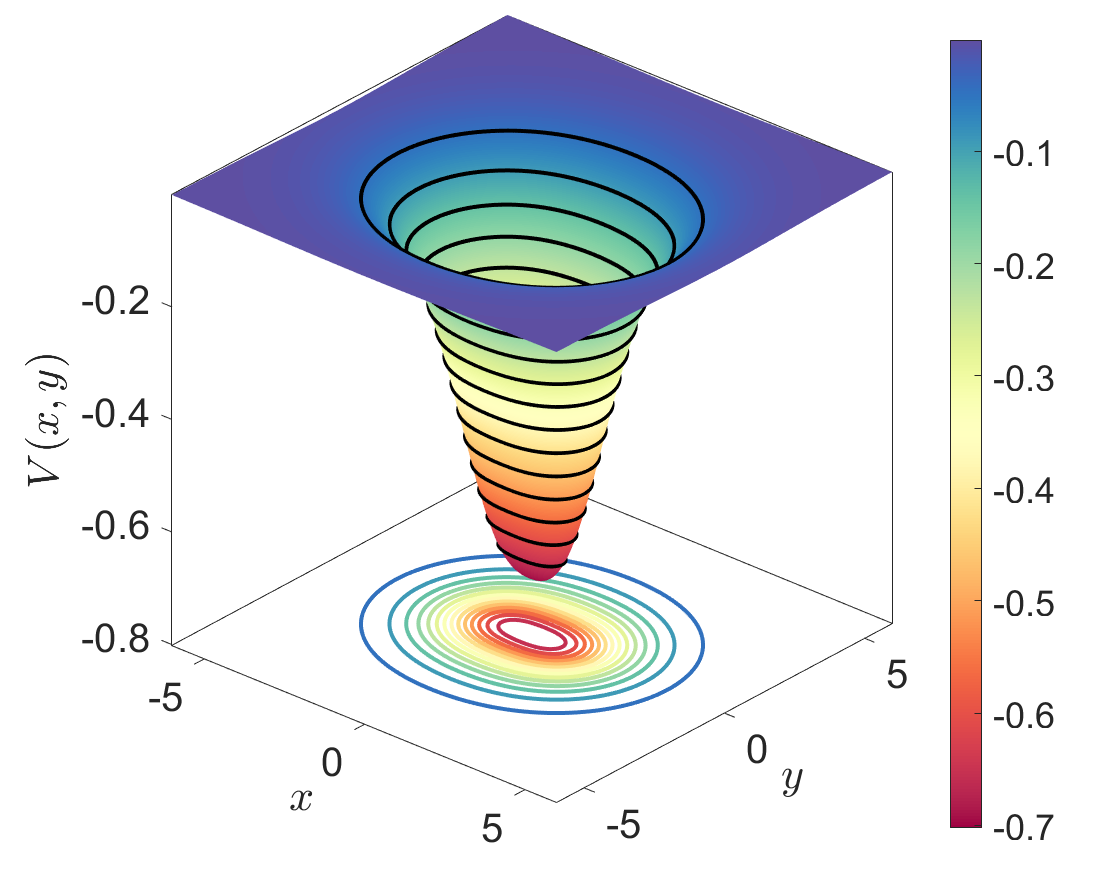
\includegraphics[scale=0.3]{untitled.png}
    \caption{Surface plot of Double-vdW potential Equation \eqref{eq:vdw-single}. Parameters used: $C_6 = 1/2$, $\alpha = 1$, $\beta = 1/8$ and $d = 1$}
    \label{fig:vdw-single_surface}
\end{figure}


\begin{figure}
    \centering
    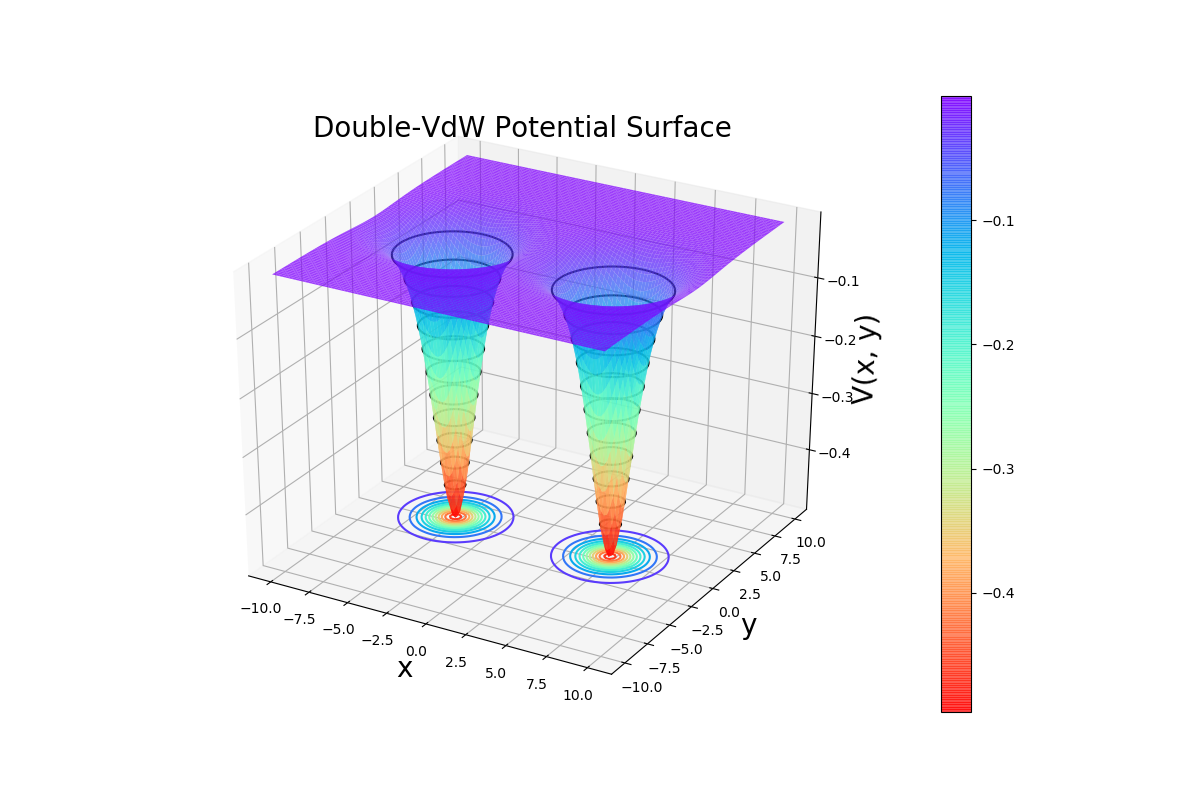
\includegraphics[scale=0.5]{notebooks/figures/double-vdw_surface.png}
    \caption{Surface plot of Double-vdW potential Equation \eqref{eq:vdw-double}. Parameters used: $C_6 = 1/2$, $\alpha = 1$, $\beta = 1/8$, and  $d = 5$ }
    \label{fig:vdw-double_surface}
\end{figure}


The two degrees-of-freedom Hamiltonian for the Cirque potential energy surface is defined as the classical sum of kinetic plus potential energy:
\begin{equation}
H(x,y,p_x,p_y) = \dfrac{p_x^2}{2 m_1} + \dfrac{p_y^2}{2 m_2} + V(x,y)
\label{eq:hamil}
\end{equation}
Hamilton's equations that determine the systems dynamical evolution are given by:
\begin{equation}
\begin{cases}
\dot{x} = \dfrac{\partial H}{\partial p_x} = \dfrac{p_x}{m_1} \\[.5cm]
\dot{y} = \dfrac{\partial H}{\partial p_y} = \dfrac{p_y}{m_2} \\
\dot{p}_x = - \dfrac{\partial H}{\partial x} = - \dfrac{\partial V}{\partial x} = - 6 \, \beta \, C_6 \left[\dfrac{x - d}{\left(\beta\left[\left(x - d\right)^2 + y^2\right] + \alpha\right)^4} + \dfrac{x + d}{\left(\beta\left[\left(x + d\right)^2 + y^2\right] + \alpha\right)^4}\right] \\[.7cm]
\dot{p}_y = - \dfrac{\partial H}{\partial y} = - \dfrac{\partial V}{\partial y} = - 6 \, \beta \, C_6 \, y \left[\dfrac{1}{\left(\beta\left[\left(x - d\right)^2 + y^2\right] + \alpha\right)^4} + \dfrac{1}{\left(\beta\left[\left(x + d\right)^2 + y^2\right] + \alpha\right)^4}\right]
\end{cases}
\label{eq:ham_eq}
\end{equation}
The equilibrium points $\mathbf{r}_e = (x_e,y_e,p_{x,e},p_{y,e})$ of the dynamical system given above are contained in configuration space, since $p_{x,e} = p_{y,e} = 0$, and they are also critical points of the PES, that is $\nabla V (x_e,y_e) = \mathbf{0}$. It is straightforward to check that these conditions give the points:
\begin{equation}
\mathbf{r}_e^{1} = (0,0,0,0) \quad,\quad \mathbf{r}_e^{2} = (-d,0,0,0) \quad,\quad \mathbf{r}_e^{3} = (d,0,0,0)
\label{eq:eq_pts}
\end{equation}
The linear stability of these equilibrium points is determined by the eigenvalues of the Jacobian matrix given by the linearization of Eq. \eqref{eq:ham_eq} about each of the points. In order to construct the Jacobian, we need to compute the second order partial derivatives that characterize the Hessian matrix of the PES:
\begin{equation}
\begin{cases}
\dfrac{\partial^{\,	2} V}{\partial x^2} = 6 \, \beta \, C_6 \left[\dfrac{\beta\left[-7\left(x - d\right)^2 + y^2\right] + \alpha}{\left(\beta\left[\left(x - d\right)^2 + y^2\right] + \alpha\right)^5} + \dfrac{\beta\left[-7\left(x + d\right)^2 + y^2\right] + \alpha}{\left(\beta\left[\left(x + d\right)^2 + y^2\right] + \alpha\right)^5} \right] \\[.8cm]

\dfrac{\partial^{\,	2} V}{\partial y^2} = 6 \, \beta \, C_6 \left[\dfrac{\beta\left[\left(x - d\right)^2 - 7 y^2\right] + \alpha}{\left(\beta\left[\left(x - d\right)^2 + y^2\right] + \alpha\right)^5} + \dfrac{\beta\left[\left(x + d\right)^2 - 7y^2\right] + \alpha}{\left(\beta\left[\left(x + d\right)^2 + y^2\right] + \alpha\right)^5} \right] \\[.8cm]

\dfrac{\partial^{\,	2} V}{\partial x \partial y} = - 48 \, \beta^2 \, C_6 \, y \left[\dfrac{x - d}{\left(\beta\left[\left(x - d\right)^2 + y^2\right] + \alpha\right)^5} + \dfrac{x + d}{\left(\beta\left[\left(x + d\right)^2 + y^2\right] + \alpha\right)^5}\right]
\end{cases}
\label{eq:second_pder}
\end{equation}

\newpage
\bibliographystyle{siam}
\bibliography{cirque}

\end{document}
